% This chapter is about word representations

\section{Introduction}

How can text-based models of word representation be improved in order to achieve human-like performance on evaluations like SimLex-999? Improved algorithms are undoubtedly part of the picture, but it is plausible that models may never acquire human-quality word representations from raw text, however efficient the learning algorithm and however much data they observe. This is because text data as a learning resource lacks various characteristics of the information available to human learners. For instance, much of conceptual acquisition and word learning, particularly at the early stages, apparently involves the unification of linguistic concepts with those acquired via the perceptual system~\citep{barsalou2005situating}. In addition, as the conceptual system develops, humans actively learn via interactions that depend on the current output of the learner, or explicit explanations targetted at the learner, or following a curriculum.Information in this form is not available to the text-based learning algorithms described in the previous chapter. 

In light of these observations, in this chapter I seek to improve the representations acquired by Neural Language Models (NLMs) by training on information sources other than raw text. The analyses focus on word representations because the corresponding models and  and evaluations are better understood, although the conclusions should ultimately extend to phrases and sentences (see Chapter~/ref{CH4}).

 I begin by exploring ways to endow word-learning models with information corresponding to that which is available to the sensory-perceptual system when humans learn concepts. Earlier studies had shown that data from images~\citep{feng2010visual,bruni2012distributional} and data corresponding to other modalities~\cite{kiela2015multi} can enrich distributed representations beyond what can be acquired from text. The analyses presented here extend these studies in two respects. First, it applies a novel algorithm for `mixing' information from different modalities, facilitated by fast NLMs and moderated by word frequency statistics in text. Second, it explicitly considers representations of abstract  (\emph{curiosity}, \emph{loyalty}) as well as concrete (\emph{cat}, \emph{dog}) words. As I show, this is particularly important for language understanding models, since abstract words are much more common than concrete words in adult language. 

In the second part of this chapter, I show how enhanced word representations can be acquired from bilingual text data, using a recently-developed deep sequence-to-sequence learning architecture trained to translate between pairs of European languages. These experiments can be understood as a (crude) cognitive model of bilingual learners, demonstrating how the need to translate between languages might influence or stimulate the acquisition of word concepts. As with the multi-modal learning in the first part of the chapter, I observed show clear quantitative and qualitative differences in word representations acquired via this bilingual learning framework compared with those acquired via equivalent means from (raw) monolingual text. Specifically, the embedding spaces acquired via this bilingual framework are orientated to reflect semantic similarity to a much greater extent than conventional monolingual representation spaces, whose organisation better reflects relatedness. 

\section{Grounded acquisition of abstract concepts from multi-modal data}

Multi-modal models that learn semantic representations from both language and information about the perceptible properties of concepts were originally motivated by parallels with human word learning \citep{andrews2009integrating} and evidence that many concepts are grounded in perception \citep{barsalou2005situating}. The perceptual information in such models is generally mined directly from images \citep{feng2010visual,bruni2012distributional} or from data collected in psychological studies \citep{silberer2012grounded,rollermultimodal}. 

By exploiting the additional information encoded in perceptual input, multi-modal models can outperform language-only models on a range of semantic NLP tasks, including modelling similarity \citep{bruni2014multimodal} and free association \citep{silberer2012grounded}, predicting compositionality \citep{rollermultimodal} and concept categorization \citep{silberer2014learning}. However, to date, this superiority has only been established when evaluating on concrete words such as \emph{house} or \emph{car}, rather than abstract concepts, such as \emph{welcome} or \emph{transport}. Indeed, differences between abstract and concrete processing and representation suggest that conclusions about concrete concept learning may not necessarily hold in the general case~\citep{paivio1991dual,hill2013quantitative}. In this paper, I therefore focus on multi-modal models for learning abstract as well as concrete concept (word) representations.

Although concrete concepts might seem more basic or fundamental, the vast majority of open-class, meaning-bearing words in everyday language are in fact abstract. 72\% of the noun or verb tokens in the British National Corpus \citep{leech1994claws4} are rated by human judges\footnote{Contributors to the USF dataset \citep{nelson2004university}} as more abstract than the noun \emph{war}, for instance, a concept many would already consider to be quite abstract. Moreover, abstract concepts by definition encode higher-level (more general) principles than concrete concepts, which typically reside naturally in a single semantic category or domain \citep{crutch2005abstract}. It is therefore likely that abstract representations may prove highly applicable for multi-task, multi-domain or transfer learning models, which aim to acquire `general-purpose' conceptual knowledge without reference to a specific objective or task \citep{collobert2008unified,mesnil2012unsupervised}. 

Motivated by these observations, I introduce an architecture for learning both abstract and concrete representations that generalizes the Skipgram model of \citep{mikolov2013efficient} from corpus-based  to multi-modal learning. The extended model is designed to reflect aspects of human word learning, in that it introduces more perceptual information about commonly-occurring concrete concepts and less information about rarer concepts. 

I train the model on running-text language and two sources of perceptual descriptors for concrete nouns: the ESPGame dataset of annotated images \citep{von2004labeling} and the CSLB set of concept property norms \citep{devereux2013centre}. I find that the model \emph{combines} information from the different modalities more effectively than previous methods, resulting in an improved ability to model the USF free association gold standard \citep{nelson2004university} for concrete nouns. In addition, the architecture  \emph{propagates} the extra-linguistic input for concrete nouns to improve representations of abstract concepts more effectively than alternative methods. While this propagation can effectively extend the advantage of the multi-modal approach to many more concepts than simple concrete nouns, I observe that the benefit of adding perceptual input appears to decrease as target concepts become more abstract. Indeed, for the most abstract concepts of all, language-only models still provide the most effective learning mechanism.  

Finally, I investigate the optimum quantity and type of perceptual input for such models. Between the most concrete concepts, which can be effectively represented directly in the perceptual modality, and the most abstract concepts, which cannot, I identify a set of concepts that cannot be represented effectively directly in the perceptual modality, but still benefit from perceptual input propagated in the model via concrete concepts. 

My motivation in designing the model and experiments in this section is both practical and theoretical. Taken together, the empirical observations I present are potentially important for optimizing the learning of representations of concrete and abstract concepts in multi-modal models. In addition, they offer a degree of insight into the poorly understood issue of how abstract concepts may be encoded in human memory.    

\subsection{Model Design}

Before describing how the multi-modal architecture encodes and integrates perceptual information, I first describe the underlying corpus-based representation learning model. 

\paragraph{Language-only model} The multi-modal architecture builds on the log-linear Skipgram model proposed by \cite{mikolov2013efficient} and described in Chapter~\ref{CH2}. Here, I extend this architecture via a simple means of introducing perceptual information that aligns with human language learning. Based on the assumption that frequency in domain-general linguistic corpora correlates with the likelihood of `experiencing' a concept in the world \citep{bybee2001frequency,chater2006probabilistic}, perceptual information is introduced to the model whenever designated concrete concepts are encountered in the running-text linguistic input. This has the effect of introducing more perceptual input for commonly experienced concrete concepts and less input for rarer concrete concepts. 

To implement this process,  perceptual information is extracted from external sources and encoded in an associative array \(\bf{P}\), which maps (typically concrete) words \(w\) to bags of perceptual features \({\bf b}(w)\). The construction of this array depends on the perceptual information source; the process for the chosen sources is detailed in Section~\ref{percep_sources}.  

Training the model begins as with the Skipgram model on running-text. When a sentence \(S_m\) containing a word \(w\) in the domain of \(\mathbf{P}\) is encountered, the model completes training on \(S_m\) and begins learning from a perceptual pseudo-sentence \(\hat{S}(w)\).  \(\hat{S_m}(w)\) is constructed  by randomly sampling features from \({\bf b}(w)\) to occupy positions before and instances of \(w\), so that  \(\hat{S_m}(w)\) is the same length as \(S_m\) (see Figure~\ref{examples}). Once training on \(\hat{S_m}(w)\) is completed, the model reverts to the next `real' (linguistic) sentence \(S_{m+1}\), and the process continues. Thus, when a concrete concept is encountered in the corpus, its embedding is first updated based on language (moved incrementally closer to concepts appearing in similar linguistic contexts), and then on perception (moved incrementally closer to concepts with the same or similar perceptual features).  

For greater flexibility, I introduce a parameter \(\alpha\) reflecting the raw quantity of perceptual information relative to linguistic input. When \(\alpha=2\), two pseudo-sentences are generated and inserted for every corpus occurrence of a token from the domain of \(\mathbf{P}\). For non-integral \(\alpha \), the number of sentences inserted is \( \lfloor \alpha \rfloor \), and a further sentence is added with probability \(\alpha - \lfloor \alpha \rfloor \).

In all experiments reported in the following sections I set the window size parameter \(k = 5\) and the minimum frequency parameter \(f = 3\), which guarantees that the model learns embeddings for all concepts in the evaluation sets. While the model learns both target and context-embeddings for each word in the vocabulary, I conduct the experiments with the target embeddings only. I set the dimension parameter \(d = 300 \) as this produces high quality embeddings in the language-only case \citep{mikolov2013efficient}. 

\begin{figure} \(\hat{S}(crocodile) =\)\small{ {\bf Crocodile} legs {\bf crocodile} teeth {\bf crocodile} teeth {\bf crocodile} scales {\bf crocodile} green {\bf crocodile}. \\ \\ \(\hat{S}(screwdriver)=\) { \bf Screwdriver} handle {\bf screwdriver} flat  {\bf screwdriver} long {\bf screwdriver}  handle {\bf screwdriver}  head. } \caption{\label{examples} Example pseudo-sentences generated for training the model.}\end{figure}

\subsection{Information sources}
\label{percep_sources}

We construct the associative array of perceptual information \(\mathbf{P}\) from two sources typical of those used for multi-modal semantic models.

\paragraph{ESPGame dataset} The ESP-Game dataset (ESP) \citep{von2004labeling} consists of 100,000 images, each annotated with a list of lexical concepts that appear in that image. For any concept \(w\) identified in an ESP image, I construct a corresponding bag of features \({\bf b}(w)\). For each ESP image \(I\) that contains \(w\), I append the other concept tokens identified in \(I\) to \({\bf b}(w)\). Thus, the more frequently a concept co-occurs with \(w\) in images, the more its corresponding lexical token occurs in \({\bf b}(w)\). The array \(\mathbf{P_{ESP}}\) in this case then consists of the  \( (w,  {\bf b}(w) ) \) pairs.

\paragraph{CSLB Property Norms} The Centre for Speech, Language and the Brain norms (CSLB) \citep{devereux2013centre} is a recently-released dataset containing semantic properties for 638 concrete concepts produced by human annotators. The CSLB dataset was compiled in the same way as the \cite{mcrae2005semantic} property norms used widely in multi-modal models \citep{silberer2012grounded,rollermultimodal}; I use CSLB because it contains more concepts. For each concept, the proportion of the 30 annotators that produced a given feature can also be employed as a measure of the strength of that feature.

When encoding the CSLB data in \(\mathbf{P}\), I first map properties to lexical forms (e.g. \emph{is\_green} becomes \emph{green}). By directly identifying perceptual features and linguistic forms in this way, I treat features observed in the perceptual data as (sub)concepts to be acquired via the same multi-modal input streams and stored in the same domain-general memory as the evaluation concepts. This non-modular characterisation of semantic memory  in fact corresponds to a view of cognition that is sometimes disputed \citep{fodor1983modularity}. In future studies I hope to compare the present approach to architectures with domain-specific conceptual memories. 

For each concept \(w\) in CSLB, I then construct a feature bag \({\bf b}(w)\) by appending lexical forms to \({\bf b}(w)\) such that the count of each feature word is equal to the strength of that feature for \(w\). Thus, when features are sampled from \({\bf b}(w)\) to create pseudo-sentences (as detailed previously) the probability of a feature word occuring in a sentence reflects feature strength. The array \(\mathbf{P_{CSLB}}\) then consists of all \( (w,  {\bf b}(w) ) \) pairs.

\paragraph{Linguistic input} The linguistic input to all models is the 400m word Text8 Corpus\footnote{From http://mattmahoney.net/dc/textdata.html} of Wikipedia text, split into sentences and with punctuation removed. 



 \begin{table}[t]\begin{center}\begin{tabular}{c|ccc|c}


\multicolumn{2}{c}{\bf ESPGame} &\multicolumn{1}{c}{} & \multicolumn{2}{c}{\bf CSLB}\\
 \underline{Image 1} &  \underline{Image 2} & &  \underline{Crocodile} & \underline{Screwdriver} \\ 
\footnotesize{red} &  \footnotesize{wreck} &  &  \footnotesize{has 4 legs (7)} &  \footnotesize{has handle (28)} \\ 
\footnotesize{chihuaua} &  \footnotesize{cyan} & &  \footnotesize{has tail (18)} &  \footnotesize{has head (5)} \\ 
\footnotesize{eyes} &  \footnotesize{man} & &  \footnotesize{has jaw (7)} & \footnotesize{is long (9)} \\ 
\footnotesize{little} &  \footnotesize{crash} & &  \footnotesize{has scales (8)} &   \footnotesize{is plastic (18)} \\ 
\footnotesize{ear} &  \footnotesize{accident} & &  \footnotesize{has teeth (20)} & \footnotesize{is metal (28)} \\ 
\footnotesize{nose}  &  \footnotesize{street} & &  \footnotesize{is green (10}) &  \\ 
\footnotesize{small} &   & & \footnotesize{is large (10)} &    \\ 






\end{tabular}\end{center}\caption{\label{font-table} Concepts identified in images in the ESP Game (left) and features produced for concepts by human annotators in the CSLB dataset (with feature strength, max=30).}\end{table}







\subsection{Evaluation}

SimLex-999 was produced after these experiments were carried out. I therefore evaluated the quality of representations by how well they reflect the University of South Florida Norms (USF) \citep{nelson2004university} free association scores. These norms measure the strenght of association between over 40,000 concept pairs, many of which, importantly, contain abstract concepts. Prior to SimLex-999, they had been widely used in NLP to evaluate semantic representations \citep{andrews2009integrating,feng2010visual,silberer2012grounded,rollermultimodal}. Each concept that I extracted from the USF database was also rated for conceptual concreteness on a Likert scale of 1-7 by at least 10 human annotators. Following previous studies \citep{huang2012improving,silberer2012grounded}, I measured the (Spearman \(\rho\)) correlation between association scores and the cosine similarity of vector representations.

 \begin{table}[t]\begin{center}\begin{tabular}{l|l|c}



\bf Concept 1 & \bf Concept 2 & \bf Assoc. \\
 \hline 
abdomen \footnotesize{ (6.83)} & stomach \footnotesize{ (6.04)} & 0.566 \\
throw \footnotesize{  (4.05)} & ball  \footnotesize{ (6.08)} & 0.234 \\
hope \footnotesize{  (1.18)} & glory \footnotesize{ (3.53)} & 0.192 \\
egg \footnotesize{ (5.79)} & milk \footnotesize{ (6.66)} & 0.012 \\



\end{tabular}\end{center}\caption{\label{font-table} Example concept pairs (with mean concreteness rating) and free-association scores from the USF dataset.}\end{table}






I created separate abstract and concrete concept lists by ranking the USF concepts according to concreteness and sampling at random from the first and fourth quartiles. I also introduced a complementary noun/verb dichotomy,\footnote{Based on the majority POS-tag of words in the lemmatized British National Corpus \citep{leech1994claws4}} on the intuition that information propagation may occur differently from noun to noun or from noun to verb (because of their distinct structural relationships in sentences). The abstract/concrete and noun/verb dichotomies yielded four distinct concept lists. For consistency, the concrete noun list was filtered so that all concrete noun concepts \(w\) have perceptual representations {\bf b}(w) in both  \(\mathbf{P_{ESP}}\) and  \(\mathbf{P_{CSLB}}\). For each of the four resulting concept lists \(C\) (concrete/abstract, noun/verb), a corresponding set of evaluation pairs  \( \{ (w_1, w_2) \in USF :  w_1, w_2 \in C\}\) was extracted (see Table~\ref{set_details} for details). 



 \begin{table}[t]\begin{center}\begin{tabular}{l|r|r|p{2.1cm}}



\bf Concept Type & \bf  List & \bf Pairs & \bf Examples \\ 

\hline concrete nouns & 541 & 1418 & \emph{yacht, cup} \\

abstract nouns & 100 & 295 & \emph{fear, respect} \\

all nouns & 666 & 1815 & \emph{fear, cup} \\

concrete verbs & 50 & 66 & \emph{kiss, launch} \\

abstract verbs & 50 & 127 & \emph{differ, obey} \\

all verbs & 100 & 221 & \emph{kiss, obey} \\

\end{tabular}\end{center}\caption{\label{set_details} Details the subsets of USF data used in the evaluations}\end{table}






\subsection{Results and Discussion}

Our experiments were designed to answer four questions, outlined in the following subsections: (1) Which model architectures perform best at \emph{combining} information pertinent to multiple modalities when such information exists explicitly (as common for concrete concepts)? (2) Which model architectures best propagate perceptual information to concepts for which it does not exist explicitly (as is common for abstract concepts)? (3) Is it preferable to include all of the perceptual input that can be obtained from a given source, or to filter this input stream in some way? (4) How much perceptual vs. linguistic input is optimal for learning various concept types? 

\subsection{Combining information sources} 
\label{conc1}
To evaluate the approach as a method of information combination I compared its performance on the concrete noun evaluation set against alternative methods. When implementing the alternatives, I first encoded the perceptual input directly into sparse feature vectors, with coordinates for each of the 2,726 features in CSLB and for each of the 100,000 images in ESP. 

The first alternative was simple concatenation of these perceptual vectors with linguistic vectors embeddings learned by the \cite{mikolov2013efficient} model on the Text8 Corpus. In the second alternative, proposed for multi-modal models by \cite{silberer2012grounded}, Canonical Correlation Analysis (CCA) \citep{hardoon2004canonical} was applied to the vectors of both modalities. This yielded reduced-dimensionality representations that preserve underlying inter-modal correlations, which are then concatenated. The final alternative, proposed by \cite{bruni2014multimodal} involved applying Singular Value Decomposition (SVD) to the matrix of concatenated multi-modal representations, yielding smoothed representations.\footnote{CCA was implemented using the \emph{CCA} package in R. SVD was implemented using the Python \emph{sparsesvd} package, with truncation factor \(k=1024\) as per \cite{bruni2014multimodal}.}

I compared these alternatives to the proposed model with \(\alpha = 1\). In The CSLB and ESP models, all training pseudo-sentences were generated from the arrays \(\mathbf{P_{CSLB}}\) and \(\mathbf{P_{ESP}}\) respectively. In the models classed as \emph{CSLB\&ESP}, a random choice between \(\mathbf{P_{CSLB}}\) and \(\mathbf{P_{ESP}}\) was made every time perceptual input was included (so that the overall quantity of perceptual information was the same). 

As shown in Figure~\ref{main_results} (left side), the embeddings learned by the model achieved a higher correlation with the USF data than simple concatenation, CCA and SVD regardless of perceptual input source. With the optimal perceptual source (ESP only), for instance, the correlation was 11\% higher that the next best alternative method, CCA. 

One possible factor behind this improvement is that, in the model, the learned representations fully integrate the two modalities, whereas for both CCA and the concatenation method each representation feature (whether of reduced dimension or not) corresponds to a particular modality. This deeper integration may help the architecture to overcome the challenges inherent in information combination such as inter-modality differences in information content and representation sparsity.   


\subsection{Propagating input to abstract concepts} 
\label{conc2}
To test the process of information propagation in the model, I evaluated the learned embeddings of more abstract concepts. I compared the approach with two recently-proposed alternative methods for inferring perceptual features when explicit perceptual information is unavailable. 

\paragraph{Johns and Jones} In the method of \cite{johns2012perceptual}, pseudo-perceptual representations for target concepts without a perceptual representations (uni-modal concepts) are inferred as a weighted average of the perceptual representations of concepts that do have such a representation (bi-modal concepts). 

In the first step of their two-step method, for each uni-modal concept  \(\bf k\), a quasi-perceptual representation is computed as an average of the perceptual representations of bi-modal concepts, weighted by the proximity between each of these concepts and \( \bf k\)\[{\bf k}^p = \sum_{{\bf c} \in \bar{C}} S({\bf k}^l,{\bf c}^l)^\lambda \cdot {\bf c}^p  \] where \(  \bar{C} \) is the set of bi-modal concepts, \({\bf c}^p\) and  \({\bf k}^p\) are the perceptual representations for \(\bf c\) and \(\bf k\) respectively, and  \({\bf c}^l\) and \({\bf k}^l\) the linguistic representations. The exponent parameter \(\lambda \) reflects the learning rate. 

In step two, the initial quasi-perceptual representations are inferred for a second time, but with the weighted average calculated over the perceptual or initial quasi-perceptual representations of all other words, not just those that were orignally bi-modal. As with \cite{johns2012perceptual}, I set the learning rate parameter \( \lambda\) to be 3 in the first step and 13 in the second.  


\paragraph{Ridge Regression} A simpler method for mixing modalities can be achieved using ridge regression. Ridge regression is a variant of least squares regression in which a regularization term is added to the training objective to favor solutions with certain properties. 

For bimodal concepts of dimension \(n_p\), I used ridge regression to learn \(n_p\) linear functions \( f_i: \mathbb{R}^{n_l} \to \mathbb{R} \) that map the linguistic representations (of dimension \(n_l\)) to a particular perceptual feature \(i\). These functions were then applied together to map the linguistic representations of uni-modal concepts to full quasi-perceptual representations.

Following~\cite{hill2014multi}, I took the Euclidian \( l_2 \) norm of the inferred parameter vector as the regularization term. This ensured that the regression favors lower coefficients and a smoother solution function, which should provide better generalization performance than simple linear regression. The objective for learning the \( f_i \) was then to minimize \[ \| {\bf a}X - Y_i \|_2^2 + \|{\bf a}\|_2^2 \] where \( {\bf a}\) is the vector of regression coefficients, \( X \) is a matrix of linguistic representations and \(  Y_i \) a vector of the perceptual feature \(i\) for the set of bi-modal concepts.

\paragraph{Comparisons} I applied the Johns and Jones method and ridge regression starting from linguistic embeddings acquired by the \cite{mikolov2013efficient} model on the Text8 Corpus, and concatenated the resulting pseudo-perceptual and linguistic representations. The perceptual input for all models was limited to concrete nouns (i.e. concrete nouns were the only bi-modal concepts in the models).

 \begin{figure*}  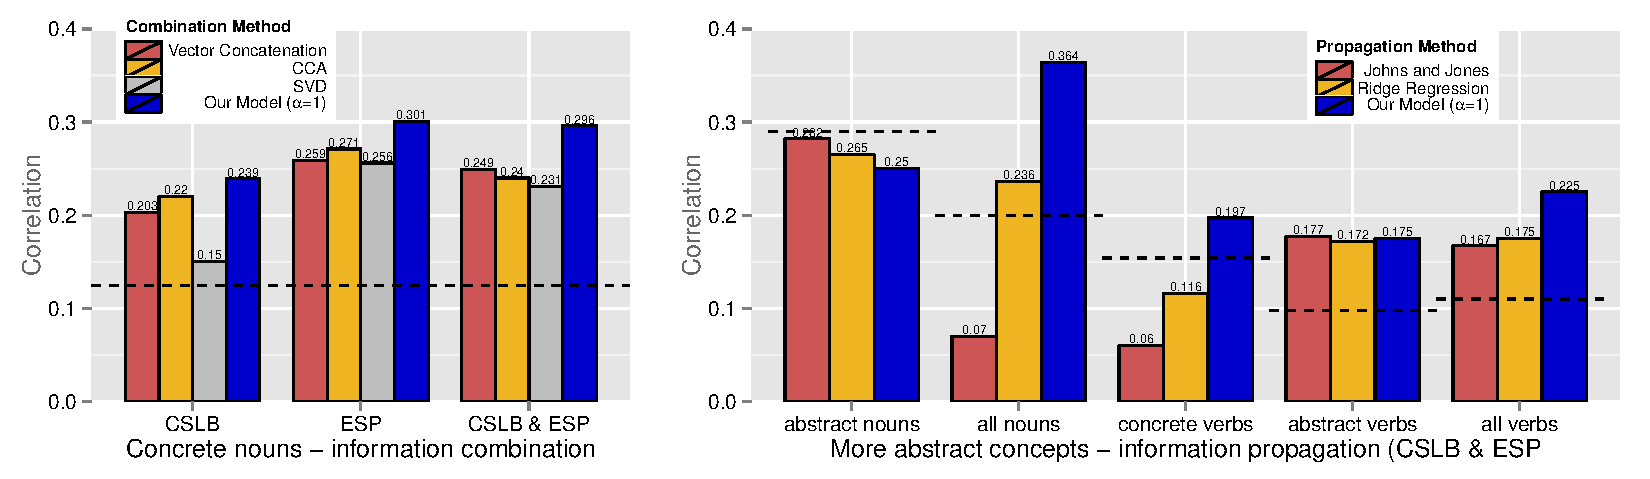
\includegraphics[width = \textwidth]{Chapter_3/Graph_1_EMNLP2014}  \caption{\label{main_results} The proposed approach compared with other methods of information combination (left) and propagation. Dashed lines indicate language-only model baseline.}\end{figure*}

Figure~\ref{main_results} (right side) illustrates the propagation performance of the three models. While the correlations overall may seem somewhat low, this is a consequence of the difficulty of modeling the USF data. In fact, the performance of both the language-only model and the multi-modal extension across the concept types, ranging from \(0.18 - 0.36\), is equal to or higher than equivalent models evaluated on the same data previously \citep{feng2010visual,silberer2012grounded,silberer2013models}. 

For learning representations of concrete verbs, the approach achieves a 69\% increase in performance over the next best alternative. The performance of the model on abstract verbs is marginally inferior to Johns and Jones' method. Nevertheless, the clear advantage for concrete verbs makes the model the best choice for learning representations of verbs in general, as shown by performance on the set \emph{all verbs}, which also includes mixed abstract-concrete pairs. 

The model is also marginally inferior to alternative approaches in learning representations of abstract nouns. However, in this case, no method improves on the linguistic-only baseline. It is possible that perceptual information is simply so removed from the core semantics of these concepts that they are best acquired via the linguistic medium alone, regardless of learning mechanism. The moderately inferior performance of the method in such cases is likely caused by its greater inherent inter-modal dependence compared with methods that simply concatenate uni-modal representations. When the perceptual signal is of low quality, this greater inter-modal dependence allows the linguistic signal to be obscured. The trade-off, however, is the higher quality joint representations when the perceptual signal is of higher-quality, exemplified by the fact that the proposed approach outperforms alternatives on the set \emph{all nouns}, which includes the more concrete nouns. 

\subsection{Direct representation vs. propagation}
\label{conc3}

 \begin{figure*}[t] 

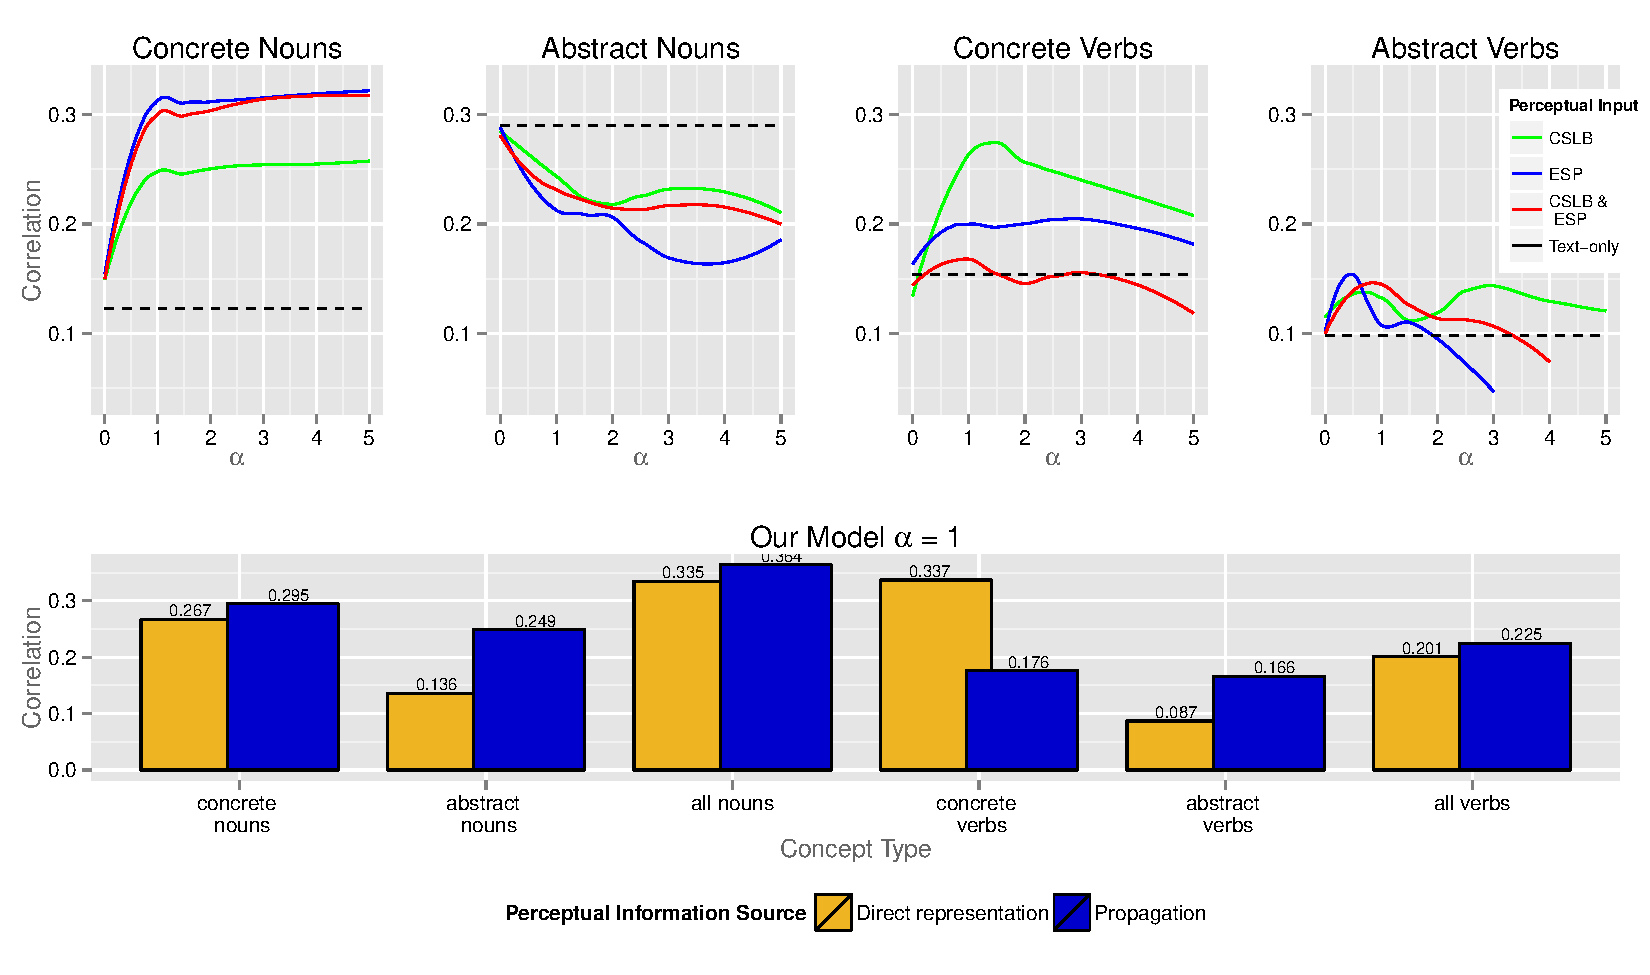
\includegraphics[width = \textwidth]{Chapter_3/Graph_2_EMNLP2014}  

\caption{\label{repprop} {\bf Top}: Comparing the strategy of directly representing abstract concepts from perceptual information where available (yellow bars) vs. propagating via concrete concepts. {\bf Bottom}: The effect of increasing \(\alpha\) on correlation with USF pairs (Spearman \(\rho\)) for each concept type. Horizontal dashed lines indicate language-only model baseline.}

\end{figure*}

Although property norm datasets such as the CSLB data typically consist of perceptual feature information for concrete nouns only, image-based datasets such as ESP do contain information on more abstract concepts, which was omitted from the previous experiments. Indeed, image banks such as Google Images contain millions of photographs portraying quite abstract concepts, such as \emph{love} or \emph{war}. On the other hand, encodings or descriptions of abstract concepts are generally more subjective and less reliable than those of concrete concepts \citep{katja2005content}. I therefore investigated whether or not it is preferable to include this additional information as model input or to restrict perceptual input to concrete nouns as previously.    

Of the evaluation sets, it was possible to construct from ESP (and add to \(\mathbf{P_{ESP}}\)) representations for all of the concrete verbs, and for approximately half of the abstract verbs and abstract nouns. Figure~\ref{repprop} (top), shows the performance of a the model trained on all available perceptual input versus the model in which the perceptual input was restricted to concrete nouns. 

The results reflect a clear manifestation of the abstract/concrete distinction. Concrete verbs behave similarly to concrete nouns, in that they can be effectively represented directly from perceptual information sources. The information encoded in these representations is beneficial to the model and increases performance. In contrast, constructing `perceptual' representations of abstract verbs and abstract nouns directly from perceptual information sources is clearly counter-productive (to the extent that performance also degrades on the combined sets \emph{all nouns} and \emph{all verbs}). It appears in these cases that the perceptual input acts to obscure or contradict the otherwise useful signal inferred from the corpus.

As shown in the previous section, the inclusion of any form of perceptual input inhibits the learning of abstract nouns. However, this is not the case for abstract verbs. Our model learns higher quality representations of abstract verbs when perceptual input is restricted to concrete nouns than when no perceptual input is included whatsoever \emph{and} when perceptual input is included for both concrete nouns and abstract verbs. This supports the idea of a gradual scale of concreteness: the most concrete concepts can be effectively represented directly in the perceptual modality; somewhat more abstract concepts cannot be represented directly in the perceptual modality, but have representations that are improved by propagating perceptual input from concrete concepts via language; and the most abstract concepts are best acquired via language alone.   

\subsection{Source and quantity of perceptual input} For different concept types, I tested the effect of varying the proportion of perceptual to linguistic input (the parameter \(\alpha\)). Perceptual input was restricted to concrete nouns as in Sections~\ref{conc1}-\ref{conc3}.

As shown in Figure~\ref{repprop}, performance on concrete nouns improves (albeit to a decreasing degree) as \( \alpha \) increases. When learning concrete noun representations, linguistic input is apparently redundant if perceptual input is of sufficient quality and quantity. For the other concept types, in each case there is an optimal value for \( \alpha \) in the range \(0.5 - 0.2\), above which perceptual input obscures the linguistic signal and performance degrades. The proximity of these optima to 1 suggests that  for optimal learning, when a concrete concept is experienced approximately equal weight should be given to available perceptual and linguistic information. 

\subsection{Conclusions}

Motivated by the notable prevalence of abstract concepts in everyday language, and their likely importance to flexible, general-purpose representation learning, this section has investigated how abstract and concrete representations can be acquired by multi-modal models. In doing so, I presented a simple and easy-to-implement architecture for acquiring semantic representations of both types of concept from linguistic and perceptual input. 

While NLMs have been applied to the problem of multi-modal representation learning previously \citep{srivastava2012multimodal,wu2013online} the model and experiments develop this work in several important ways. First, I addressed the problem of learning abstract concepts. By isolating concepts of different concreteness and part-of-speech in the evaluation sets, and separating the processes of information combination and propagation, I demonstrate that the multi-modal approach is indeed effective for some, but perhaps not all, abstract concepts. In addition, the model introduces a clear parallel with human language learning. Perceptual input is introduced precisely when concrete concepts are `experienced' by the model in the corpus text, much like a language learner experiencing concrete entities via sensory perception.  

Taken together, the findings indicate the utility of distinguishing three concept types when learning representations in the multi-modal setting. 

\paragraph{Type I} Concepts that can be effectively represented directly in the perceptual modality. For such concepts, generally concrete nouns or concrete verbs, the proposed approach provides a simple means of combining perceptual and linguistic input. The resulting multi-modal representations are of higher quality than those learned via other approaches, resulting in a performance improvement of over 10\% in modelling free association.

\paragraph{Type II} Concepts, including abstract verbs, that cannot be effectively represented directly in the perceptual modality, but whose representations can be improved by joint learning from linguistic input and perceptual information about related concepts. Our model can effectively propagate perceptual input (exploiting the relations inferred from the linguistic input) from Type I concepts to enhance the representations of Type II concepts above the language-only baseline. Because of the frequency of abstract concepts, such propagation extends the benefit of the multi-modal approach to a far wider range of language than models based solely in the concrete domain. 

\paragraph{Type III} Concepts, such as abstract nouns, which are more effectively learned via language-only models than multi-modal models. Neither the model I introduce here nor other proposed propagation methods achieve an improvement in representation quality for these concepts over the language-only baseline. Of course, it is an empirical question whether a multi-modal approach could ever enhance the representation learning of these concepts, one with potential implications for cognitive theories of grounding (a topic of much debate in psychology \citep{grafton2009embodied,barsalou2010grounded}). 

Additionally, I investigated the optimum type and quantity of perceptual input for learning concepts of different types. I showed that too much perceptual input can result in degraded representations. For concepts of type I and II, the optimal quantity resulted from setting \(\alpha = 1\); i.e. whenever a concrete concept was encountered, the model learned from an equal number of language-based and perception-based examples. While I make no formal claims here, such observations may ultimately provide insight into human language learning and semantic memory. 

% \section{Multi-modal fusion based on image dispersion}

% include your own bib file like this:


\section{Learning word representations from bilingual data using encoder-decoder models}

Recent empirical~\citep{baroni2014don,levy2015improving} and theoretical~\citep{levy2014neural} studies have yielded a better understanding of how log-linear NLMs such as Skipgram and CBOW acquire meaningful conceptual semantics. However, much less is known about the word embeddings learned by deeper NLMs with more nuanced or complex objectives. In this section, I take some steps in this direction by considering the embeddings learned by architectures with a very different objective function to the Skipgram or CBOW models: \emph{neural machine translation} (NMT) \emph{models}. NMT models have recently emerged as an alternative to statistical, phrase-based translation models, and are beginning to achieve impressive translation performance~\citep{kalchbrenner13emnlp,devlin2014fast,Sutskever2014sequence}.

We show that NMT models are not only a potential new direction for machine translation, but are also an effective means of learning word embeddings. Specifically, NMT word embeddings encode information relating to conceptual similarity (rather than non-specific relatedness or association) and lexical syntactic role more effectively than embeddings from monolingual NLMs. I demonstrate that these properties persist when translating between different language pairs (English-French and English-German). Further, based on the observation of subtle language-specific effects in the embedding spaces, I conjecture as to why similarity dominates over other semantic relations in translation embedding spaces. Finally, I discuss a potential limitation of the application of NMT models for embedding learning - the computational cost of training large vocabularies of embeddings - and show that a novel method for overcoming this issue preserves the aforementioned properties of translation-based embeddings. 

% I show that the precise information encoFinally, I consider ways to combine the distinct information encoded in language-model embeddings and those from translation embeddings. And I consider ways to overcome two important limitations of neural translation models as embedding-learning architectures: the computational difficulty in learning large vocabularies of embeddings, and the requirement for sentence-aligned bilingual training corpora.   

\subsection{Neural Machine Translation Models}

The objective of NMT models is to generate an appropriate sentence in a target language \(S_t\)  given a sentence \(S_s\) in the source language (see e.g.~\citep{kalchbrenner13emnlp,Sutskever2014sequence}). As a by-product of learning to meet this objective, NMT models learn distinct sets of embeddings for the vocabularies \(V_ s\) and \(V_t\) in the source and target languages respectively.

Observing a training case \((S_s, S_t)\), these models represent \(S_s\) as an ordered sequence of embeddings of words from \(V_s\). The sequence for \(S_s\) is then encoded into a single representation \(R_S\).\footnote{Alternatively, subsequences (phrases) of \(S_s\) may be encoded at this stage in place of the whole sentence~\citep{bahdanau2014neural}.} Finally, by referencing the embeddings in \(V_t\), \(R_S\) and a representation of what has been generated thus far, the model decodes a sentence in the target language word by word. If at any stage the decoded word does not match the corresponding word in the training target \(S_t\), the error is recorded. The weights and embeddings in the model, which together parameterise the encoding and decoding process, are updated based on the accumulated error once the sentence decoding is complete. 

Although NMT models can differ in their low-level architecture~\citep{kalchbrenner13emnlp,Cho2014,bahdanau2014neural}, the translation objective exerts similar pressure on the word embeddings in all cases. The source language embeddings must be such that the model can combine them to form single representations for ordered sequences of multiple words (which in turn must enable the decoding process). The target language embeddings must facilitate the process of decoding these representations into correct target-language sentences.    

\subsection{Other bilingual models of learning word representations}
Before the advent of effective end-to-end NMT systems, several models had been developed with the specific goal of acquiring distributed word representations from bilingual corpora, aligned at the document, paragraph or word level~\citep{Haghighi2008Learning,vulic2011identifying,mikolov2013exploiting,Hermann:2014:ICLR,lauly2014autoencoder}. While these approaches rely on the same training data as NMT models, one important difference is that they represent the words from two different languages in single common vector space so that words in one language are close to words with similar or related meanings in the other (this is not the case for NMT models, where the source and target language word embeddings inhabit distinct vector spaces). The resulting multilingual embedding spaces have been effectively applied to bilingual lexicon extraction~\citep{Haghighi2008Learning,vulic2011identifying,mikolov2013exploiting} and document classification~\citep{Klementiev,Hermann:2014:ICLR,lauly2014autoencoder,Kocisky:2014}.

For comparison, we focus on two representatives of this class of (non-NMT) bilingual model. The first is that of \cite{Hermann:2014:ICLR}, whose embeddings improve on the performance of~\cite{Klementiev} in document classification applications. As with NMT models, this model can be trained directly on bitexts aligned only at the sentence rather than word level. When training, for aligned sentences \(S_E\) and \(S_F\) in different languages, the model computes representations \(R_E\) and \(R_F\) by summing the embeddings of the words in \(S_E\) and \(S_F\) respectively. The embeddings are then updated to minimise the divergence between \(R_E\) and \(R_F\) (since they convey a common meaning). A noise-contrastive loss function ensures that the model does not arrive at trivial (e.g. all zero) solutions to this objective.~\cite{Hermann:2014:ICLR} show that, despite the lack of prespecified word alignments, words in the two languages with similar meanings converge in the bilingual embedding space.\footnote{The models of \cite{lauly2014autoencoder} and \cite{Hermann:2014:ICLR} both aim to minimise the divergence between source and target language sentences represented as sums of word embeddings. Because of these similarities, I do not compare with both in this paper.}

The second model I examine is that of \cite{faruqui2014improving}. Unlike the models described above, \cite{faruqui2014improving} showed explicitly that projecting word embeddings from two languages (learned independently) into a common vector space can favourably influence the orientation of word embeddings when considered in their monolingual subspace; i.e relative to other words in their own language. In contrast to the other models considered in this paper, the approach of~\cite{faruqui2014improving} requires bilingual data to be aligned at the word level.

\subsection{Experiments}

To learn translation-based embeddings, I trained two different NMT models. The first is the RNN encoder-decoder, \emph{RNNenc}~\citep{Cho2014}, which uses a recurrent neural network (RNN) to encode all of the source sentence into a single vector on which the decoding process is conditioned. The second is the \emph{RNN Search} architecture~\citep{bahdanau2014neural}, which was designed to overcome limitations exhibited by the RNN encoder-decoder when translating very long sentences. RNN Search includes an \emph{attention} mechanism, an additional feed-forward network that learns to attend to different parts of the source sentence when decoding each word in the target sentence.\footnote{Access to source code and limited GPU time prevented me from training and evaluating the embeddings from other NMT models such as that of~\cite{kalchbrenner13emnlp},~\cite{devlin2014fast} and \cite{Sutskever2014sequence}. The underlying principles of encoding-decoding also apply to these models, and I expect the embeddings would exhibit similar properties to those analysed here.} Both models were trained on a 348m word corpus of English-French sentence pairs or a 91m word corpus of English-German sentence pairs.\footnote{These corpora were produced from the WMT ’14 parallel data after conducting the data-selection procedure described by~\cite{Cho2014}. } 

To explore the properties of bilingual embeddings learned via objectives other than direct translation, I trained the \emph{BiCVM} model of~\cite{Hermann:2014:ICLR} on the same data, and also downloaded the projected embeddings of~\cite{faruqui2014improving}, \emph{FD}, trained on a bilingual corpus of comparable size (\(\approx 300\) million words per language).\footnote{Available from \url{http://www.cs.cmu.edu/~mfaruqui/soft.html}. The available embeddings were trained on English-German aligned data, but the authors report similar to for English-French.} Finally, to compare with monolingual word embedding models, I trained a conventional skipgram model~\citep{mikolov2013distributed} and its \emph{Glove} variant~\citep{Pennington2014} for the same number of epochs on the English half of the bilingual corpus. 

To analyse the effect on embedding quality of increasing the quantity of training data, I then trained the monolingual models on increasingly large random subsamples of Wikipedia text (up to a total of 1.1bn words). Lastly, I extracted embeddings from a full-sentence language model, \emph{CW},~\citep{collobert2008unified}, which was trained for several months on the same Wikipedia 1bn word corpus. Note that increasing the volume of training data for the bilingual (and NMT) models was not possible because of the limited size of available sentence-aligned bitexts. 
 
\subsubsection{Similarity and relatedness modelling}

As in previous studies~\citep{Agirre2009,bruni2014multimodal,baroni2014don}, the initial evaluations involved calculating pairwise (cosine) distances between embeddings and correlating these distances with (gold-standard) human judgements of the strength of relationships between concepts. For this I used three different gold standards: WordSim-353~\citep{Agirre2009}, MEN~\citep{bruni2014multimodal} and SimLex-999~\citep{hill2014simlex}. Recall that there is a clear distinction between WordSim-353 and MEN, on the one hand, and SimLex-999, on the other, in terms of the semantic relationship that they quantify. For both WordSim-353 and MEN, annotators were asked to rate how \emph{related} or \emph{associated} two concepts are. Consequently, pairs such as [\emph{clothes}-\emph{closet}], which are clearly related but ontologically dissimilar, have high ratings in WordSim-353 and MEN. In contrast, such pairs receive a low rating in SimLex-999, where only genuinely \emph{similar} concepts, such as [\emph{coast}- \emph{shore}], receive high ratings. 

Table~\ref{table:perf} shows the correlations of NMT (English-French) embeddings, other bilingually trained embeddings and monolingual embeddings with these three lexical gold-standards. NMT outperform monolingual embeddings, and, to a lesser extent, the other bilingually trained embeddings, on SimLex-999. However, this clear advantage is not observed on MEN and WordSim-353, where the projected embeddings of~\cite{faruqui2014improving}, which were tuned for high performance on WordSim-353, perform best. Given the aforementioned differences between the evaluations, this suggests that bilingually-trained embeddings, and NMT based embeddings in particular, better capture similarity, whereas monolingual embedding spaces are orientated more towards relatedness. 

\begin{table}[t]
\begin{center}
\begin{tabular}{r c | r  r  r  | r r | r r |}
\multicolumn{2}{c|}{~} &\multicolumn{3}{c|}{Monolingual models}  & \multicolumn{2}{c|}{\small Biling. models} & \multicolumn{2}{c|}{NMT models}\\  
    \multicolumn{2}{c|}{~} &\bf Skipgram &\bf Glove &\bf CW & \bf FD & \bf BiCVM & \bf RNNenc &\bf RNNsearch \\ 
\hline
WordSim-353   & \(\rho\) & 0.52 & 0.55 & 0.51 &{\bf  0.69} & 0.50 &   0.57 &  0.58 \\
MEN & \(\rho\) & 0.44 & 0.71 & 0.60 & {\bf 0.78} & 0.45 &  0.63 &  0.62  \\
\hdashline
SimLex-999 & \(\rho\) & 0.29 & 0.32 & 0.28 & 0.39 & 0.36 &   {\bf 0.52} &  0.49 \\
SimLex-333 & \(\rho\) &  018&0.18  &0.07  & 0.24  &  0.34 & { \bf 0.49}   & 0.45   \\
TOEFL & \(\%\) & 0.75 & 0.78 & 0.64 & 0.84 & 0.87 &  {\bf 0.93} &  {\bf 0.93} \\
Syn/antonym & \(\%\) & 0.69  & 0.72  &  0.75 & 0.76 & 0.70 &  {\bf 0.79} & 0.74 \\
\end{tabular}
\caption{ NMT embeddings (RNNenc and RNNsearch) clearly outperform alternative embedding-learning architectures on tasks that require modelling similarity (below the dashed line), but not on tasks that reflect relatedness. Bilingual embedding spaces learned without the translation objective are somewhere between these two extremes.}
\label{table:perf}
\end{center}
\vspace{-5mm}
\end{table}


\begin{table}[t]
\begin{center}
\begin{tabular}{r | r  r  r | r r | r r}
&\bf Skipgram &\bf Glove &\bf CW&\bf FD &\bf BiCVM  &\bf RNNenc &\bf RNNsearch \\ 
\hline
\emph{teacher}  & {\small \emph{vocational}} &  {\small \emph{student}} 
& {\small \emph{student}} &{\small \emph{elementary}} & {\small  \emph{faculty}} & {\small \emph{professor}}  & {\small \emph{instructor}} \\ 
 & {\small \emph{in-service}} &  {\small \emph{pupil}} 
& {\small \emph{tutor}} & {\small \emph{school}}& {\small  \emph{professors}} & {\small \emph{instructor}}  & {\small \emph{professor}} \\ 
 & {\small \emph{college}} &  {\small \emph{university}} 
& {\small \emph{mentor}} & {\small \emph{classroom}}& {\small \emph{teach}}& {\small \emph{trainer}}  & {\small \emph{educator}} \\ 
\hdashline
\emph{eaten}  & {\small \emph{spoiled}} &  {\small \emph{cooked}} 
&  {\small \emph{baked}} &{\small \emph{ate}}& {\small  \emph{eating}}& {\small \emph{ate}} & {\small \emph{ate}} \\ 
  & {\small \emph{squeezed}} &  {\small \emph{eat}} 
&  {\small \emph{peeled}} &{\small \emph{meal}}& {\small \emph{eat}}& {\small \emph{consumed}} & {\small \emph{consumed}} \\ 
  & {\small \emph{cooked}} &  {\small \emph{eating}} 
&  {\small \emph{cooked}} &{\small \emph{salads}}& {\small \emph{baking}}& {\small \emph{tasted}} & {\small \emph{eat}} \\ 
\hdashline
\emph{Britain}  & {\small \emph{Northern}} &  {\small \emph{Ireland}} 
& {\small \emph{Luxembourg}} &{\small \emph{UK}}& {\small \emph{UK}} & {\small  \emph{UK}} & {\small \emph{England}} \\ 
& {\small \emph{Great}} &  {\small \emph{Kingdom}} 
& {\small \emph{Belgium}} &{\small \emph{British}}& {\small \emph{British}} & {\small  \emph{British}} & {\small \emph{UK}} \\ 
 & {\small \emph{Ireland}} &  {\small \emph{Great}} 
& {\small \emph{Madrid}} &{\small \emph{London}}& {\small \emph{England}} & {\small  \emph{America}} & {\small \emph{Syria}} \\ 


\end{tabular}
\caption{Nearest neighbours (excluding plurals) in the embedding spaces of different models. All models were trained for 6 epochs on the translation corpus except CW and FD (as noted previously). NMT embedding spaces are oriented according to similarity, whereas embeddings learned by monolingual models are organized according to relatedness. The other bilingual model BiCVM also exhibits a notable focus on similarity.}
\label{table:neigh}
\end{center}
\vspace{-5mm}
\end{table}

To test this hypothesis further, I ran three more evaluations designed to probe the sensitivity of models to similarity as distinct from relatedness or association. In the first, I measured performance on SimLex-Assoc-333 ~\citep{hill2014simlex}. This evaluation comprises the 333 most related pairs in SimLex-999, according to an independent empirical measure of relatedness (free associate generation~\citep{nelson2004university}). Importantly, the pairs in SimLex-Assoc-333, while all strongly related, still span the full range of similarity scores.\footnote{The most dissimilar pair in SimLex-Assoc-333 is [\emph{shrink,grow}] with a score of 0.23. The highest is [\emph{vanish},\emph{disappear}] with 9.80.} Therefore, the extent to which embeddings can model this data reflects their sensitivity to the similarity (or dissimilarity) of two concepts, even in the face of a strong signal in the training data that those concepts are related.    

The TOEFL synonym test is another similarity-focused evaluation of embedding spaces. This test contains 80 cue words, each with four possible answers, of which one is a correct synonym~\citep{landauer1997solution}. I computed the proportion of questions answered correctly by each model, where a model's answer was the nearest (cosine) neighbour to the cue word in its vocabulary.\footnote{To control for different vocabularies, I restricted the effective vocabulary of each model to the intersection of all model vocabularies, and excluded all questions that contained an answer outside of this intersection.} Note that, since TOEFL is a test of synonym recognition, it necessarily requires models to recognise similarity as opposed to relatedness.  

Finally, I tested how well different embeddings enabled a supervised classifier to distinguish between synonyms and antonyms, since synonyms are necessarily similar and people often find antonyms, which are necessarily dissimilar, to be strongly associated. For 744 word pairs hand-selected as either synonyms or antonyms,\footnote{Available online at \url{http://www.cl.cam.ac.uk/~fh295/}.} I presented a Gaussian SVM with the concatenation of the two word embeddings. I evaluated accuracy using 10-fold cross-validation. 

As shown in Table~\ref{table:perf}, with these three additional similarity-focused tasks the same pattern of results is observed. NMT embeddings outperform other bilingually-trained embeddings which in turn outperform monolingual models. The difference is particularly striking on SimLex-Assoc-333, which suggests that the ability to discern similarity from relatedness (when relatedness is high) is perhaps the most clear distinction between the bilingual spaces and those of monolingual models. 

These conclusions are also supported by qualitative analysis of the various embedding spaces. As shown in Table~\ref{table:neigh}, in the NMT embedding spaces the nearest neighbours (by cosine distance) to concepts such as \emph{teacher} are genuine synonyms such as \emph{professor} or \emph{instructor}. The bilingual objective also seems to orientate the non-NMT embeddings towards semantic similarity, although some purely related neighbours are also oberved. In contrast, in the monolingual embedding spaces the neighbours of \emph{teacher} include  highly related but dissimilar concepts such as \emph{student} or \emph{college}. 

%\footnote{Readers can inspect nearest neighbours in each embedding space using the web demo.} 
 
\subsubsection{Importance of training data quantity}

In previous work, monolingual models were trained on corpora many times larger than the English half of the parallel translation corpus. Indeed, the ability to scale to large quantities of training data was one of the principal motivations behind the skipgram architecture~\citep{mikolov2013distributed}. To check if monolingual models simply need more training data to capture similarity as effectively as bilingual models, I therefore trained them on increasingly large subsets of Wikipedia.\footnote{We did not do the same for the translation models because sentence-aligned bilingual corpora of comparable size do not exist.} As shown in Figure~\ref{fig:size}, this is not in fact the case. The performance of monolingual embeddings on similarity tasks remains well below the level of the NMT embeddings and somewhat lower than the non-MT bilingual embeddings as the amount of training data increases. 

\begin{figure*}[h]
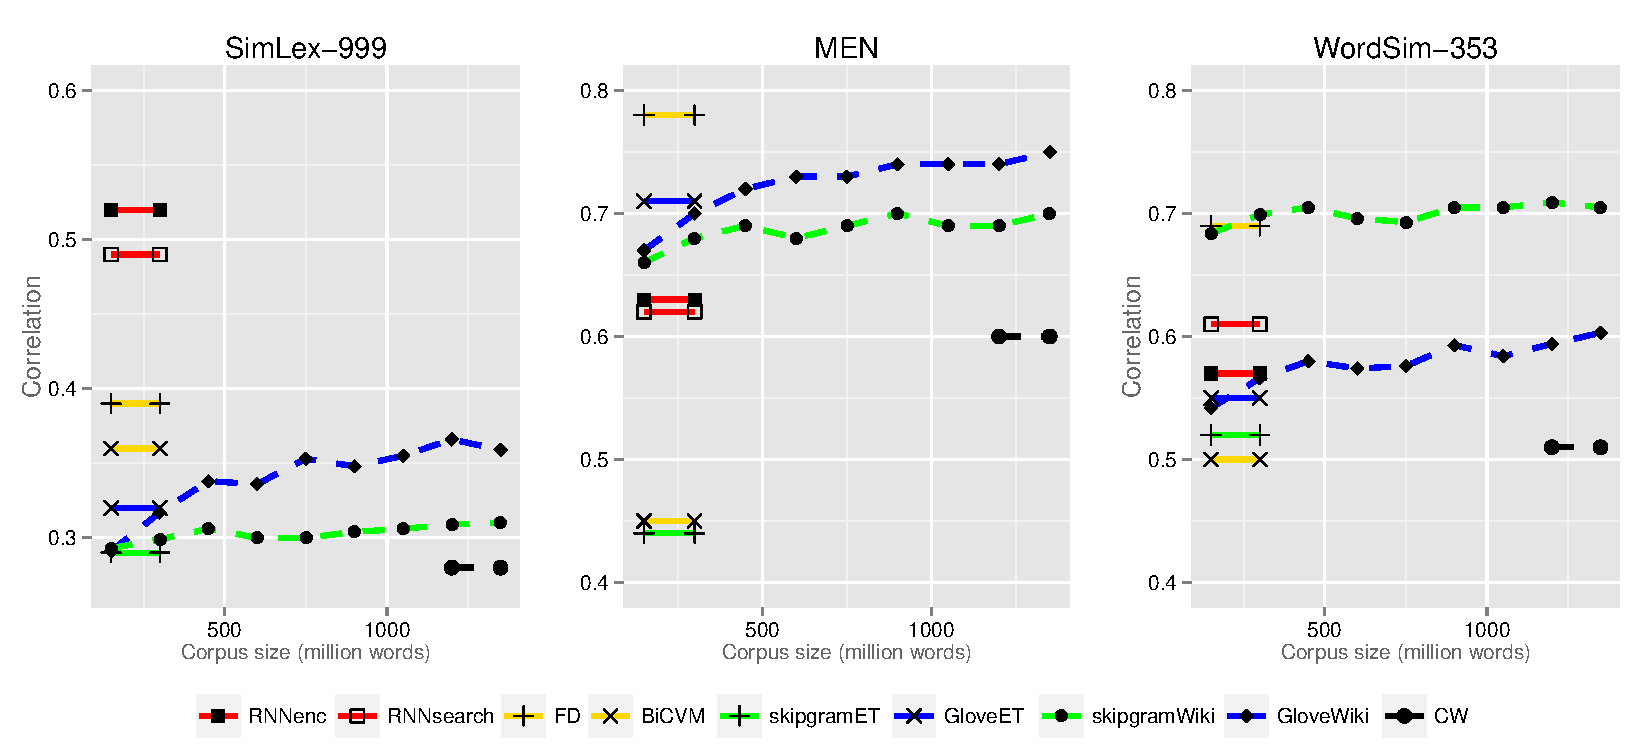
\includegraphics[width = \textwidth,clip=True,trim=0 10 0 10]{Chapter_3/Figure_1_ICLR2015}
\vspace{-4mm}
\caption{The effect of increasing the amount of training data on the quality of monolingual embeddings, based on similarity-based evaluations (SimLex-999) and two relatedness-based evaluations (MEN and WordSim-353). \emph{ET} in the legend indicates models trained on the English half of the translation corpus. \emph{Wiki} indicates models trained on Wikipedia.}
\label{fig:size}
\end{figure*}


\subsubsection{Analogy resolution}

Lexical analogy questions have been used as an alternative way of evaluating word representations. In this task, models must identify the correct answer (\emph{girl}) when presented with analogy questions such as `\emph{man} is to \emph{boy} as \emph{woman} is to ?'. It has been shown that Skipgram-style models are surprisingly effective at answering such questions~\citep{mikolov2013distributed}. This is because, if \( \bf m, b \) and \( \bf w\) are skigram-style embeddings for \emph{man}, \emph{boy} and \emph{woman} respectively, the correct answer is often the nearest neighbour in the vocabulary (by cosine distance) to the vector \( \bf v = w + b - m \). 

We evaluated embeddings on analogy questions using the same vector-algebra method as~\cite{mikolov2013distributed}. As in the previous section, for fair comparison I excluded questions containing a word outside the intersection of all model vocabularies, and restricted all answer searches to this reduced vocabulary. This left 11,166 analogies. Of these, 7219 are classed as `syntactic', in that they exemplify mappings between parts-of-speech or syntactic roles (e.g. \emph{fast} is to \emph{fastest} as \emph{heavy} is to \emph{heaviest}), and 3947 are classed as `semantic` (\emph{Ottawa} is to \emph{Canada} as \emph{Paris} is to \emph{France}), since successful answering seems to rely on some (world) knowledge of the concepts themselves. 

As shown in Fig.~\ref{fig:analogy}, NMT embeddings yield relatively poor answers to semantic analogy questions compared with monolingual embeddings and the bilingual embeddings \emph{FD} (which are projections of similar monolingual embeddings).\footnote{The performance of the FD embeddings on this task is higher than that reported by~\cite{faruqui2014improving} because I search for answers over a smaller total candidate vocabulary.} It appears that the translation objective prevents the embedding space from developing the same linear, geometric regularities as skipgram-style models with respect to semantic organisation. This also seems to be true of the embeddings from the full-sentence language model \emph{CW}. Further, in the case of the Glove and FD models this advantage seems to be independent of both the domain and size of the training data, since embeddings from these models trained on only the English half of the translation corpus still outperform the translation embeddings. 

On the other hand, NMT embeddings are effective for answering syntactic analogies using the vector algebra method. They perform comparably to or even better than monolingual embeddings when trained on less data (albeit bilingual data). It is perhaps unsurprising that the translation objective incentivises the encoding of a high degree of lexical syntactic information, since coherent target-language sentences could not be generated without knowledge of the parts-of-speech, tense or case of its vocabulary items. The connection between the translation objective and the embedding of lexical syntactic information is further supported by the fact that embeddings learned by the bilingual model BiCVM do not perform comparably on the syntactic analogy task. In this model, sentential semantics is transferred via a bag-of-words representation, presumably rendering the precise syntactic information less important.

When considering the two properties of NMT embeddings highlighted by these experiments, namely the encoding of semantic similarity and lexical syntax, it is worth noting that items in the similarity-focused evaluations of the previous section (SimLex-999 and TOEFL) consist of word groups or pairs that have identical syntactic role. Thus, even though lexical semantic information is in general pertinent to conceptual similarity~\citep{levy2014dependency}, the lexical syntactic and conceptual properties of translation embeddings are in some sense independent of one another.  


\begin{figure*}[ht]

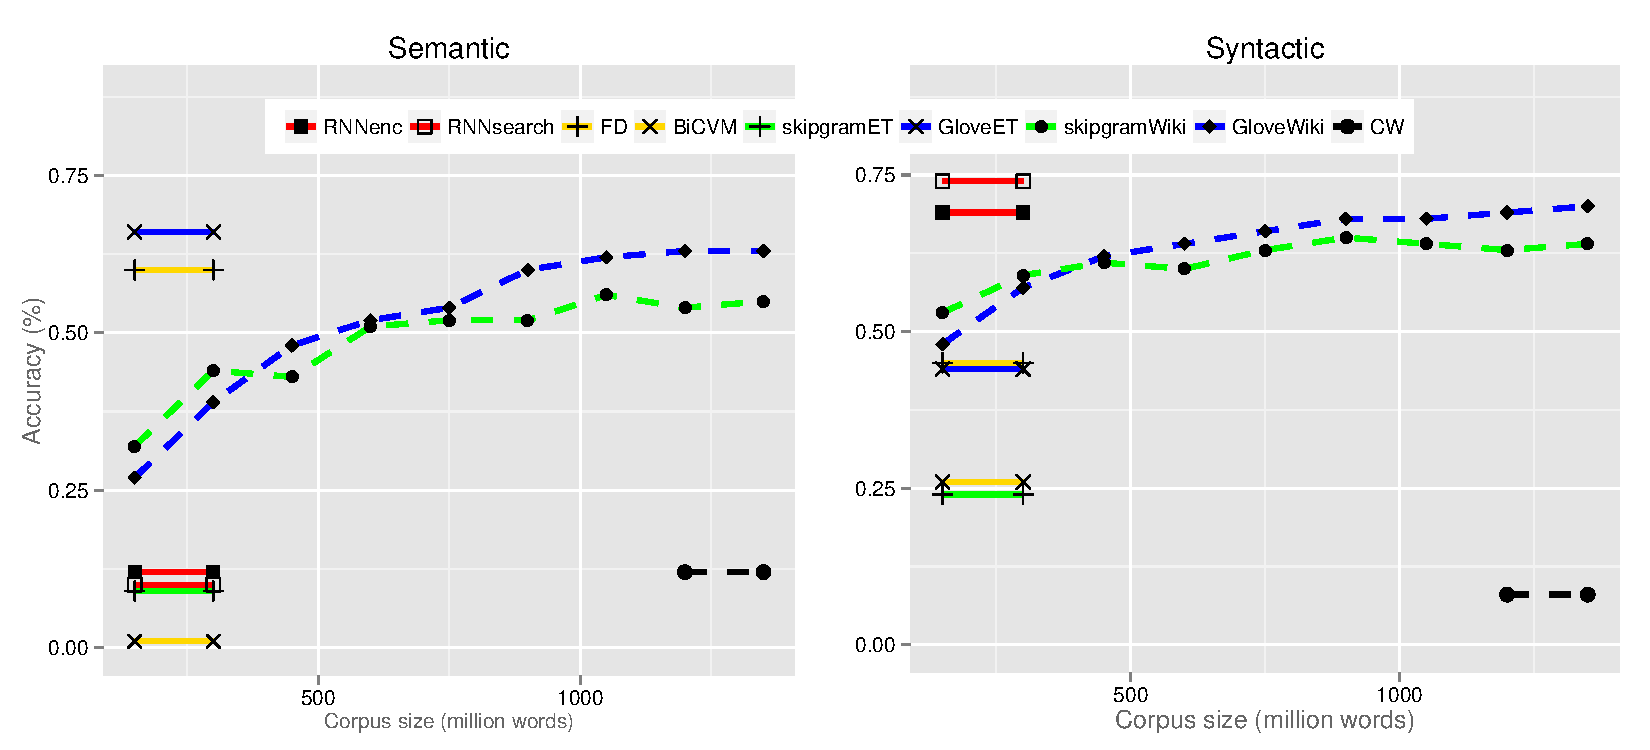
\includegraphics[width = \textwidth,clip=True,trim=0 10 0 10]{Chapter_3/Figure_2_ICLR2015}

\vspace{-4mm}
\caption{Translation-based embeddings perform best on syntactic analogies (\emph{run,ran: hide, hid}). Monolingual skipgram/Glove models are better at semantic analogies (\emph{father, man; mother, woman})}
\label{fig:analogy}

\end{figure*}

\section{Effect of Target Language}
\label{lang_effects}

To better understand why a translation objective yields embedding spaces with particular properties, I trained the RNN Search architecture to translate from English to German. 

\begin{table}[ht]
\begin{center}
\begin{tabular}{r c | m{0.9cm}  m{0.9cm}  r c c c }
    \multicolumn{2}{c|}{~} &\bf  \small EN-FR &\bf  \small EN-DE &  &  `earned' & `castle' & `money'\\ 
\cline{1-4} \cline{6-8}
WordSim-353   & \(\rho\) & 0.60 & \bf 0.61 &   & {\small \emph{gained}} & {\small \emph{chateau}} & {\small \bf \emph{ silver}} \\
MEN & \(\rho\) & 0.61 & \bf 0.62 \bf & \bf \small  EN-FR  & {\small \bf \emph{won}} & {\small \emph{palace}} & {\small \emph{funds}} \\
SimLex-999 & \(\rho\) & 0.49 &  \bf 0.50 &  & {\small \emph{acquired}}  & {\small \emph{fortress}}  & {\small \emph{cash}} \\
\cline{6-8}
SimLex-Assoc-333 & \(\rho\) & 0.45  & \bf 0.47   &   &  &   \\
TOEFL & \(\%\) & 0.90 & \bf 0.93  & &  {\small \emph{gained}}&  {\small \emph{chateau}} &  {\small \emph{funds}} \\ 
Syn/antonym & \(\%\) & \bf 0.72 &  0.70  &  \bf \small EN-DE   &  {\small \emph{deserved}}    &  {\small \emph{palace}}    &  {\small \emph{cash}} \\ 
Syntactic analogies & \(\%\) & \bf 0.73 & 0.62   &  &  {\small \emph{accummulated}}   &  {\small \bf \emph{ padlock}}   &  {\small \emph{resources}} \\  
Semantic analogies & \(\%\) & 0.10 & \bf  0.11  \\
\end{tabular}
\caption{Comparison of embeddings learned by RNN Search models translating between English-French (EN-FR) and English-German (EN-DE) on all semantic evaluations (left) and nearest neighbours of selected cue words (right). Bold italics indicate target-language-specific effects. Evaluation items and vocabulary searches were restricted to words common to both models. }
\label{table:de}
\end{center}
\vspace{-5mm}
\end{table}

As shown in Table~\ref{table:de} (left side), the performance of the source (English) embeddings learned by this model was comparable to that of those learned by the English-to-French model on all evaluations, even though the English-German training corpus (91 million words) was notably smaller than the English-French corpus (348m words). This evidence shows that the desirable properties of translation embeddings highlighted thus far are not particular to English-French translation, and can also emerge when translating to a different language family, with different word ordering conventions.     

\subsection{Overcoming the vocabulary size problem}

A potential drawback to using NMT models for learning word embeddings is the computational cost of training such a model on large vocabularies. To generate a target language sentence, NMT models repeatedly compute a softmax distribution over the target vocabulary. This computation scales with vocabulary size and must be repeated for each word in the output sentence, so that training models with large output vocabularies is challenging. Moreover, while the same computational bottleneck does not apply to the encoding process or source vocabulary, there is no way in which a translation model could learn a high quality source embedding for a word if the plausible translations were outside its vocabulary. Thus, limitations on the size of the target vocabulary effectively limit the scope of NMT models as representation-learning tools. This contrasts with the shallower monolingual and bilingual representation-learning models considered in this paper,  which efficiently compute a distribution over a large target vocabulary using either a hierarchical softmax~\citep{morin2005hierarchical} or approximate methods such as negative sampling~\citep{mikolov2013distributed,Hermann:2014:ICLR}, and thus can learn large vocabularies of both source and target embeddings.

A recently proposed solution to this problem enables NMT models to be trained with larger target vocabularies (and hence larger meaningful source vocabularies) at comparable computational cost to training with a small target vocabulary~\citep{Jean}. The algorithm uses (biased) importance sampling~\citep{Bengio+Senecal-2003-small} to approximate the probability distribution of words over a large target vocabulary with a finite set of distributions over subsets of that vocabulary. Despite this element of approximation in the decoder, extending the effective target vocabulary in this way significantly improves translation performance, since the model can make sense of more sentences in the training data and encounters fewer unknown words at test time. In terms of representation learning, the method provides a means to scale up the NMT approach to vocabularies as large as those learned by monolingual models. However, given that the method replaces an exact calculation with an approximate one, I tested how the quality of source embeddings is affected by scaling up the target language vocabulary in this way. 

\begin{table}[t]
\begin{center}
\begin{tabular}{r c | c c c c }
    \multicolumn{2}{c|}{~} &\bf RNN Search &\bf RNN Search & \bf RNN Search-LV  & \bf RNN Search-LV  \\ 
 \multicolumn{2}{c|}{~} &\bf \small EN-FR &\bf \small  EN-DE & \bf  \small EN-FR & \bf \small EN-DE \\ 
\hline
WordSim-353   & \(\rho\) & 0.60 & \bf 0.61 & 0.59 & 0.57  \\
MEN & \(\rho\) & 0.61 & \bf 0.62 & \bf 0.62 & 0.61 \\
SimLex-999 & \(\rho\) & 0.49 & 0.50 & \bf  0.51 & 0.50  \\
SimLex-Assoc-333 & \(\rho\) & 0.45  & \bf 0.47  & \bf 0.47  & 0.46   \\
TOEFL & \(\%\) & 0.90 & 0.93 & 0.93 & \bf 0.98  \\
Syn/antonym & \(\%\) & 0.72 &  0.70 & \bf 0.74 & 0.71 \\
Syntactic analogies & \(\%\) & \bf 0.73 &  0.62 & 0.71 & 0.62\\
Semantic analogies & \(\%\) & 0.10 &  0.11 & 0.08 & \bf 0.13\
\end{tabular}
\caption{Comparison of embeddings learned by the original (RNN Search - 30k French words, 50k German words) and extended-vocabulary (RNN Search-LV -500k words) models translating from English to French (EN-FR) and from English to German (EN-DE). For fair comparisons, all evaluations were restricted to the intersection of all model vocabularies.}
\label{table:ex}
\end{center}
\vspace{-5mm}
\end{table}

As shown in Table~\ref{table:ex}, there is no significant degradation of embedding quality when scaling to large vocabularies with using the approximate decoder. Note that for a fair comparison I filtered these evaluations to only include items that are present in the smaller vocabulary. Thus, the numbers do not directly reflect the quality of the additional 470k embeddings learned by the extended vocabulary models, which one would expect to be lower since they are words of lower frequency. All embeddings can be downloaded from \url{http://www.cl.cam.ac.uk/~fh295/}, and the embeddings from the smaller vocabulary models can be interrogated at \url{http://lisa.iro.umontreal.ca/mt-demo/embs/}.\footnote{A different solution to the rare-word problem was proposed by~\cite{luong2014addressing}. I do not evaluate the effects on the resulting embeddings of this method because I lack access to the source code.} 


\subsection{How similarity emerges in NMT embeddings}
\label{section:exp}

Although NMT models appear to encode both conceptual similarity and syntactic information for any source and target languages, it is not the case that embedding spaces will always be identical. Interrogating the nearest neighbours of the source embedding spaces of the English-French and English-German models reveals occasional language-specific effects. As shown in Table~\ref{table:de} (right side), the neighbours for the word \emph{earned} in the English-German model are as one might expect, whereas the neighbours from the English-French model contain the somewhat unlikely candidate \emph{won}. In a similar vein, while the neighbours of the word \emph{castle} from the English-French model are unarguably similar, the neighbours from the English-German model contain the word \emph{padlock}.
 
These infrequent but striking differences between the English-German and English-French source embedding spaces indicate how similarity might emerge effectively in NMT models. Tokens of the French verb \emph{gagner} have (at least) two possible English translations (\emph{win} and \emph{earn}). Since the translation model, which has limited encoding capacity, is trained to map tokens of \emph{win} and \emph{earn} to the same place in the target embedding space, it is efficient to move these concepts closer in the source space. Since \emph{win} and \emph{earn} map directly to two different verbs in German, this effect is not observed. On the other hand, the English nouns \emph{castle} and \emph{padlock} translate to a single noun (\emph{Schloss}) in German, but different nouns in French. Thus, \emph{padlock} and \emph{castle} are only close in the source embeddings from the English-German model. 

Based on these considerations, I can conjecture that the following condition on the semantic configuration between two language is crucial to the effective induction of lexical similarity. 

\MyQuote{\emph{For \(s_1\) and \(s_2\) in the source language, there is some \(t\) in the targThe horse raced past the barn fellet language such that there are sentences in the training data in which \(s_1\) translates to \(t\) and sentences in which \(s_2\) translates to \(t\).}}

{\centering \emph{if and only if} \\}

\MyQuote{\emph{\(s_1\) and \(s_2\) are semantically similar.}}

Of course, this condition is not true in general. However, I propose that the extent to which it holds over all possible word pairs corresponds to the quality of similarity induction in the translation embedding space. Note that strong polysemy in the target language, such as \emph{gagner = win, earn}, can lead to cases in which \(1\) is satisfied but \(2\) is not. The conjecture claims that these cases are detrimental to the quality of the embedding space (at least with regards to similarity). In practice, qualitative analyses of the embedding spaces and native speaker intuitions suggest that such cases are comparatively rare. Moreover, when such cases are observed, \(s_1\) and \(s_2\), while perhaps not similar, are not strongly dissimilar. This could explain why related but strongly dissimilar concepts such as antonym pairs do not converge in the translation embedding space. This is also consistent with qualitative evidence presented by~\cite{faruqui2014improving} that projecting monolingual embeddings into a bilingual space orientates them to better reflect the synonymy/antonymy distinction.
    

\subsection{Conclusions}

In this work, I have shown that the embedding spaces from neural machine translation models are orientated more towards conceptual similarity than those of monolingual models, and that translation embedding spaces also reflect richer lexical syntactic information. To perform well on similarity evaluations such as SimLex-999, embeddings must distinguish information pertinent to what concepts \emph{are} (their function or ontology) from information reflecting other non-specific inter-concept relationships. Concepts that are strongly related but dissimilar, such as antonyms, are particularly challenging in this regard~\citep{hill2014simlex}. Consistent with the qualitative observation made by~\cite{faruqui2014improving}, I suggested how the nature of the semantic correspondence between the words in languages enables NMT embeddings to distinguish synonyms and antonyms and, more generally, to encode the information needed to reflect human intuitions of similarity.   

The language-specific effects I observed in Section~\ref{lang_effects} suggest a potential avenue for improving translation and multi-lingual embeddings in future work. First, as the availability of fast GPUs for training grows, I would like to explore the embeddings learned by NMT models that translate between much more distant language pairs such as English-Chinese or English-Arabic. For these language pairs, the word alignment will less monotonic and may result in even more important semantic and syntactic information being encoded in the lexical representation. Further,  as observed by both~\cite{Hermann:2014:ICLR} and~\cite{faruqui2014improving}, the bilingual representation learning paradigm can be naturally extended to update representations based on correspondences between multiple languages (for instance by interleaving English-French and English-German training examples). Such an approach should smooth out language-specific effects, leaving embeddings that encode only language-agnostic conceptual semantics and are thus more generally applicable. Another related challenge is to develop smaller or less complex representation-learning tools that encode similarity with as much fidelity as NMT models but without the computational overhead. One promising approach for this is to learn word alignments and word embeddings jointly~\citep{Kocisky:2014}. This approach is effective for cross-lingual document classification, although the authors do evaluate the monolingual subspace induced by the model.

\section{Discussion}

Not all word embeddings learned from text are born equal. Depending on the application, those learned by NMT models may have particularly desirable properties. For decades, distributional semantic models have aimed to exploit Firth's famous \emph{distributional hypothesis} to induce word meanings from (monolingual) text. However, the hypothesis also betrays the weakness of the monolingual distributional approach when it comes to learning humah-quality concept representations. For while it is undeniable that ``words which are similar in meaning appear in similar distributional contexts"~\citep{dist}, the converse assertion, which is what really matters, is only sometimes true. 


